\begin{figure}[h!]
	\centering
	
	
	
	\tikzset{every picture/.style={line width=0.75pt}} %set default line width to 0.75pt        
	
	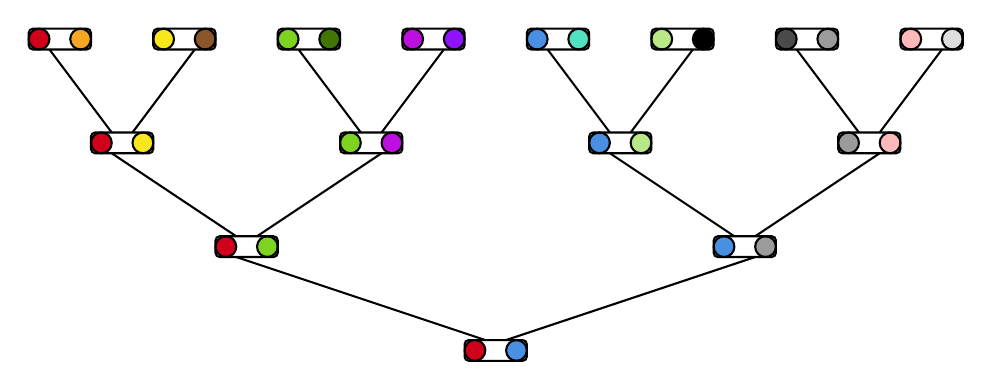
\begin{tikzpicture}[x=0.75pt,y=0.75pt,yscale=-1,xscale=1]
		%uncomment if require: \path (0,300); %set diagram left start at 0, and has height of 300
		
		%Shape: Circle [id:dp018560429656511612] 
		\draw  [fill={rgb, 255:red, 208; green, 2; blue, 27 }  ,fill opacity=1 ] (30,35) .. controls (30,32.24) and (32.24,30) .. (35,30) .. controls (37.76,30) and (40,32.24) .. (40,35) .. controls (40,37.76) and (37.76,40) .. (35,40) .. controls (32.24,40) and (30,37.76) .. (30,35) -- cycle ;
		%Shape: Circle [id:dp7337912233966392] 
		\draw  [fill={rgb, 255:red, 245; green, 166; blue, 35 }  ,fill opacity=1 ] (50,35) .. controls (50,32.24) and (52.24,30) .. (55,30) .. controls (57.76,30) and (60,32.24) .. (60,35) .. controls (60,37.76) and (57.76,40) .. (55,40) .. controls (52.24,40) and (50,37.76) .. (50,35) -- cycle ;
		%Shape: Circle [id:dp8820103548322037] 
		\draw  [fill={rgb, 255:red, 248; green, 231; blue, 28 }  ,fill opacity=1 ] (90,35) .. controls (90,32.24) and (92.24,30) .. (95,30) .. controls (97.76,30) and (100,32.24) .. (100,35) .. controls (100,37.76) and (97.76,40) .. (95,40) .. controls (92.24,40) and (90,37.76) .. (90,35) -- cycle ;
		%Shape: Circle [id:dp25856942342321] 
		\draw  [fill={rgb, 255:red, 139; green, 87; blue, 42 }  ,fill opacity=1 ] (110,35) .. controls (110,32.24) and (112.24,30) .. (115,30) .. controls (117.76,30) and (120,32.24) .. (120,35) .. controls (120,37.76) and (117.76,40) .. (115,40) .. controls (112.24,40) and (110,37.76) .. (110,35) -- cycle ;
		%Shape: Circle [id:dp5015647413644816] 
		\draw  [fill={rgb, 255:red, 126; green, 211; blue, 33 }  ,fill opacity=1 ] (150,35) .. controls (150,32.24) and (152.24,30) .. (155,30) .. controls (157.76,30) and (160,32.24) .. (160,35) .. controls (160,37.76) and (157.76,40) .. (155,40) .. controls (152.24,40) and (150,37.76) .. (150,35) -- cycle ;
		%Shape: Circle [id:dp8355950995019352] 
		\draw  [fill={rgb, 255:red, 65; green, 117; blue, 5 }  ,fill opacity=1 ] (170,35) .. controls (170,32.24) and (172.24,30) .. (175,30) .. controls (177.76,30) and (180,32.24) .. (180,35) .. controls (180,37.76) and (177.76,40) .. (175,40) .. controls (172.24,40) and (170,37.76) .. (170,35) -- cycle ;
		%Shape: Circle [id:dp5894386008313285] 
		\draw  [fill={rgb, 255:red, 189; green, 16; blue, 224 }  ,fill opacity=1 ] (210,35) .. controls (210,32.24) and (212.24,30) .. (215,30) .. controls (217.76,30) and (220,32.24) .. (220,35) .. controls (220,37.76) and (217.76,40) .. (215,40) .. controls (212.24,40) and (210,37.76) .. (210,35) -- cycle ;
		%Shape: Circle [id:dp024305607815882757] 
		\draw  [fill={rgb, 255:red, 144; green, 19; blue, 254 }  ,fill opacity=1 ] (230,35) .. controls (230,32.24) and (232.24,30) .. (235,30) .. controls (237.76,30) and (240,32.24) .. (240,35) .. controls (240,37.76) and (237.76,40) .. (235,40) .. controls (232.24,40) and (230,37.76) .. (230,35) -- cycle ;
		%Shape: Circle [id:dp03984017434261167] 
		\draw  [fill={rgb, 255:red, 74; green, 144; blue, 226 }  ,fill opacity=1 ] (270,35) .. controls (270,32.24) and (272.24,30) .. (275,30) .. controls (277.76,30) and (280,32.24) .. (280,35) .. controls (280,37.76) and (277.76,40) .. (275,40) .. controls (272.24,40) and (270,37.76) .. (270,35) -- cycle ;
		%Shape: Circle [id:dp9533983432265577] 
		\draw  [fill={rgb, 255:red, 80; green, 227; blue, 194 }  ,fill opacity=1 ] (290,35) .. controls (290,32.24) and (292.24,30) .. (295,30) .. controls (297.76,30) and (300,32.24) .. (300,35) .. controls (300,37.76) and (297.76,40) .. (295,40) .. controls (292.24,40) and (290,37.76) .. (290,35) -- cycle ;
		%Shape: Circle [id:dp18181536377245977] 
		\draw  [fill={rgb, 255:red, 184; green, 233; blue, 134 }  ,fill opacity=1 ] (330,35) .. controls (330,32.24) and (332.24,30) .. (335,30) .. controls (337.76,30) and (340,32.24) .. (340,35) .. controls (340,37.76) and (337.76,40) .. (335,40) .. controls (332.24,40) and (330,37.76) .. (330,35) -- cycle ;
		%Shape: Circle [id:dp9332038408547695] 
		\draw  [fill={rgb, 255:red, 0; green, 0; blue, 0 }  ,fill opacity=1 ] (350,35) .. controls (350,32.24) and (352.24,30) .. (355,30) .. controls (357.76,30) and (360,32.24) .. (360,35) .. controls (360,37.76) and (357.76,40) .. (355,40) .. controls (352.24,40) and (350,37.76) .. (350,35) -- cycle ;
		%Shape: Circle [id:dp7948209727823257] 
		\draw  [fill={rgb, 255:red, 74; green, 74; blue, 74 }  ,fill opacity=1 ] (390,35) .. controls (390,32.24) and (392.24,30) .. (395,30) .. controls (397.76,30) and (400,32.24) .. (400,35) .. controls (400,37.76) and (397.76,40) .. (395,40) .. controls (392.24,40) and (390,37.76) .. (390,35) -- cycle ;
		%Shape: Circle [id:dp783065963134683] 
		\draw  [fill={rgb, 255:red, 155; green, 155; blue, 155 }  ,fill opacity=1 ] (410,35) .. controls (410,32.24) and (412.24,30) .. (415,30) .. controls (417.76,30) and (420,32.24) .. (420,35) .. controls (420,37.76) and (417.76,40) .. (415,40) .. controls (412.24,40) and (410,37.76) .. (410,35) -- cycle ;
		%Shape: Circle [id:dp9591673568458936] 
		\draw  [fill={rgb, 255:red, 222; green, 222; blue, 222 }  ,fill opacity=1 ] (470,35) .. controls (470,32.24) and (472.24,30) .. (475,30) .. controls (477.76,30) and (480,32.24) .. (480,35) .. controls (480,37.76) and (477.76,40) .. (475,40) .. controls (472.24,40) and (470,37.76) .. (470,35) -- cycle ;
		%Shape: Circle [id:dp33226220726603506] 
		\draw  [fill={rgb, 255:red, 253; green, 185; blue, 186 }  ,fill opacity=1 ] (450,35) .. controls (450,32.24) and (452.24,30) .. (455,30) .. controls (457.76,30) and (460,32.24) .. (460,35) .. controls (460,37.76) and (457.76,40) .. (455,40) .. controls (452.24,40) and (450,37.76) .. (450,35) -- cycle ;
		%Shape: Circle [id:dp35016757564359635] 
		\draw  [fill={rgb, 255:red, 208; green, 2; blue, 27 }  ,fill opacity=1 ] (60,85) .. controls (60,82.24) and (62.24,80) .. (65,80) .. controls (67.76,80) and (70,82.24) .. (70,85) .. controls (70,87.76) and (67.76,90) .. (65,90) .. controls (62.24,90) and (60,87.76) .. (60,85) -- cycle ;
		%Shape: Circle [id:dp512895469837635] 
		\draw  [fill={rgb, 255:red, 248; green, 231; blue, 28 }  ,fill opacity=1 ] (80,85) .. controls (80,82.24) and (82.24,80) .. (85,80) .. controls (87.76,80) and (90,82.24) .. (90,85) .. controls (90,87.76) and (87.76,90) .. (85,90) .. controls (82.24,90) and (80,87.76) .. (80,85) -- cycle ;
		%Shape: Circle [id:dp24158056124358096] 
		\draw  [fill={rgb, 255:red, 189; green, 16; blue, 224 }  ,fill opacity=1 ] (200,85) .. controls (200,82.24) and (202.24,80) .. (205,80) .. controls (207.76,80) and (210,82.24) .. (210,85) .. controls (210,87.76) and (207.76,90) .. (205,90) .. controls (202.24,90) and (200,87.76) .. (200,85) -- cycle ;
		%Shape: Circle [id:dp7433507102379519] 
		\draw  [fill={rgb, 255:red, 74; green, 144; blue, 226 }  ,fill opacity=1 ] (300,85) .. controls (300,82.24) and (302.24,80) .. (305,80) .. controls (307.76,80) and (310,82.24) .. (310,85) .. controls (310,87.76) and (307.76,90) .. (305,90) .. controls (302.24,90) and (300,87.76) .. (300,85) -- cycle ;
		%Shape: Circle [id:dp5457939712929744] 
		\draw  [fill={rgb, 255:red, 184; green, 233; blue, 134 }  ,fill opacity=1 ] (320,85) .. controls (320,82.24) and (322.24,80) .. (325,80) .. controls (327.76,80) and (330,82.24) .. (330,85) .. controls (330,87.76) and (327.76,90) .. (325,90) .. controls (322.24,90) and (320,87.76) .. (320,85) -- cycle ;
		%Shape: Circle [id:dp6496558896089931] 
		\draw  [fill={rgb, 255:red, 155; green, 155; blue, 155 }  ,fill opacity=1 ] (420,85) .. controls (420,82.24) and (422.24,80) .. (425,80) .. controls (427.76,80) and (430,82.24) .. (430,85) .. controls (430,87.76) and (427.76,90) .. (425,90) .. controls (422.24,90) and (420,87.76) .. (420,85) -- cycle ;
		%Shape: Circle [id:dp694541172242149] 
		\draw  [fill={rgb, 255:red, 253; green, 185; blue, 186 }  ,fill opacity=1 ] (440,85) .. controls (440,82.24) and (442.24,80) .. (445,80) .. controls (447.76,80) and (450,82.24) .. (450,85) .. controls (450,87.76) and (447.76,90) .. (445,90) .. controls (442.24,90) and (440,87.76) .. (440,85) -- cycle ;
		%Shape: Circle [id:dp23498844467125868] 
		\draw  [fill={rgb, 255:red, 126; green, 211; blue, 33 }  ,fill opacity=1 ] (180,85) .. controls (180,82.24) and (182.24,80) .. (185,80) .. controls (187.76,80) and (190,82.24) .. (190,85) .. controls (190,87.76) and (187.76,90) .. (185,90) .. controls (182.24,90) and (180,87.76) .. (180,85) -- cycle ;
		%Shape: Circle [id:dp4425871714694546] 
		\draw  [fill={rgb, 255:red, 208; green, 2; blue, 27 }  ,fill opacity=1 ] (120,135) .. controls (120,132.24) and (122.24,130) .. (125,130) .. controls (127.76,130) and (130,132.24) .. (130,135) .. controls (130,137.76) and (127.76,140) .. (125,140) .. controls (122.24,140) and (120,137.76) .. (120,135) -- cycle ;
		%Shape: Circle [id:dp9851828104343108] 
		\draw  [fill={rgb, 255:red, 126; green, 211; blue, 33 }  ,fill opacity=1 ] (140,135) .. controls (140,132.24) and (142.24,130) .. (145,130) .. controls (147.76,130) and (150,132.24) .. (150,135) .. controls (150,137.76) and (147.76,140) .. (145,140) .. controls (142.24,140) and (140,137.76) .. (140,135) -- cycle ;
		%Shape: Circle [id:dp4867150146389979] 
		\draw  [fill={rgb, 255:red, 74; green, 144; blue, 226 }  ,fill opacity=1 ] (360,135) .. controls (360,132.24) and (362.24,130) .. (365,130) .. controls (367.76,130) and (370,132.24) .. (370,135) .. controls (370,137.76) and (367.76,140) .. (365,140) .. controls (362.24,140) and (360,137.76) .. (360,135) -- cycle ;
		%Shape: Circle [id:dp5602345094194735] 
		\draw  [fill={rgb, 255:red, 155; green, 155; blue, 155 }  ,fill opacity=1 ] (380,135) .. controls (380,132.24) and (382.24,130) .. (385,130) .. controls (387.76,130) and (390,132.24) .. (390,135) .. controls (390,137.76) and (387.76,140) .. (385,140) .. controls (382.24,140) and (380,137.76) .. (380,135) -- cycle ;
		%Shape: Circle [id:dp6108233873273292] 
		\draw  [fill={rgb, 255:red, 208; green, 2; blue, 27 }  ,fill opacity=1 ] (240,185) .. controls (240,182.24) and (242.24,180) .. (245,180) .. controls (247.76,180) and (250,182.24) .. (250,185) .. controls (250,187.76) and (247.76,190) .. (245,190) .. controls (242.24,190) and (240,187.76) .. (240,185) -- cycle ;
		%Shape: Circle [id:dp1579928794236467] 
		\draw  [fill={rgb, 255:red, 74; green, 144; blue, 226 }  ,fill opacity=1 ] (260,185) .. controls (260,182.24) and (262.24,180) .. (265,180) .. controls (267.76,180) and (270,182.24) .. (270,185) .. controls (270,187.76) and (267.76,190) .. (265,190) .. controls (262.24,190) and (260,187.76) .. (260,185) -- cycle ;
		%Rounded Rect [id:dp5882832862836306] 
		\draw   (30,32) .. controls (30,30.9) and (30.9,30) .. (32,30) -- (58,30) .. controls (59.1,30) and (60,30.9) .. (60,32) -- (60,38) .. controls (60,39.1) and (59.1,40) .. (58,40) -- (32,40) .. controls (30.9,40) and (30,39.1) .. (30,38) -- cycle ;
		%Rounded Rect [id:dp9713191422102239] 
		\draw   (60,82) .. controls (60,80.9) and (60.9,80) .. (62,80) -- (88,80) .. controls (89.1,80) and (90,80.9) .. (90,82) -- (90,88) .. controls (90,89.1) and (89.1,90) .. (88,90) -- (62,90) .. controls (60.9,90) and (60,89.1) .. (60,88) -- cycle ;
		%Rounded Rect [id:dp02465769539320728] 
		\draw   (120,132) .. controls (120,130.9) and (120.9,130) .. (122,130) -- (148,130) .. controls (149.1,130) and (150,130.9) .. (150,132) -- (150,138) .. controls (150,139.1) and (149.1,140) .. (148,140) -- (122,140) .. controls (120.9,140) and (120,139.1) .. (120,138) -- cycle ;
		%Rounded Rect [id:dp9965309694264901] 
		\draw   (240,182) .. controls (240,180.9) and (240.9,180) .. (242,180) -- (268,180) .. controls (269.1,180) and (270,180.9) .. (270,182) -- (270,188) .. controls (270,189.1) and (269.1,190) .. (268,190) -- (242,190) .. controls (240.9,190) and (240,189.1) .. (240,188) -- cycle ;
		%Rounded Rect [id:dp5969169663270096] 
		\draw   (360,132) .. controls (360,130.9) and (360.9,130) .. (362,130) -- (388,130) .. controls (389.1,130) and (390,130.9) .. (390,132) -- (390,138) .. controls (390,139.1) and (389.1,140) .. (388,140) -- (362,140) .. controls (360.9,140) and (360,139.1) .. (360,138) -- cycle ;
		%Rounded Rect [id:dp16634674951870254] 
		\draw   (420,82) .. controls (420,80.9) and (420.9,80) .. (422,80) -- (448,80) .. controls (449.1,80) and (450,80.9) .. (450,82) -- (450,88) .. controls (450,89.1) and (449.1,90) .. (448,90) -- (422,90) .. controls (420.9,90) and (420,89.1) .. (420,88) -- cycle ;
		%Rounded Rect [id:dp8311089140028687] 
		\draw   (300,82) .. controls (300,80.9) and (300.9,80) .. (302,80) -- (328,80) .. controls (329.1,80) and (330,80.9) .. (330,82) -- (330,88) .. controls (330,89.1) and (329.1,90) .. (328,90) -- (302,90) .. controls (300.9,90) and (300,89.1) .. (300,88) -- cycle ;
		%Rounded Rect [id:dp2800971901686894] 
		\draw   (180,82) .. controls (180,80.9) and (180.9,80) .. (182,80) -- (208,80) .. controls (209.1,80) and (210,80.9) .. (210,82) -- (210,88) .. controls (210,89.1) and (209.1,90) .. (208,90) -- (182,90) .. controls (180.9,90) and (180,89.1) .. (180,88) -- cycle ;
		%Rounded Rect [id:dp24349528888760885] 
		\draw   (90,32) .. controls (90,30.9) and (90.9,30) .. (92,30) -- (118,30) .. controls (119.1,30) and (120,30.9) .. (120,32) -- (120,38) .. controls (120,39.1) and (119.1,40) .. (118,40) -- (92,40) .. controls (90.9,40) and (90,39.1) .. (90,38) -- cycle ;
		%Rounded Rect [id:dp9906986931845275] 
		\draw   (150,32) .. controls (150,30.9) and (150.9,30) .. (152,30) -- (178,30) .. controls (179.1,30) and (180,30.9) .. (180,32) -- (180,38) .. controls (180,39.1) and (179.1,40) .. (178,40) -- (152,40) .. controls (150.9,40) and (150,39.1) .. (150,38) -- cycle ;
		%Rounded Rect [id:dp7389050829805387] 
		\draw   (210,32) .. controls (210,30.9) and (210.9,30) .. (212,30) -- (238,30) .. controls (239.1,30) and (240,30.9) .. (240,32) -- (240,38) .. controls (240,39.1) and (239.1,40) .. (238,40) -- (212,40) .. controls (210.9,40) and (210,39.1) .. (210,38) -- cycle ;
		%Rounded Rect [id:dp045791522556513864] 
		\draw   (270,32) .. controls (270,30.9) and (270.9,30) .. (272,30) -- (298,30) .. controls (299.1,30) and (300,30.9) .. (300,32) -- (300,38) .. controls (300,39.1) and (299.1,40) .. (298,40) -- (272,40) .. controls (270.9,40) and (270,39.1) .. (270,38) -- cycle ;
		%Rounded Rect [id:dp8895447163857301] 
		\draw   (330,32) .. controls (330,30.9) and (330.9,30) .. (332,30) -- (358,30) .. controls (359.1,30) and (360,30.9) .. (360,32) -- (360,38) .. controls (360,39.1) and (359.1,40) .. (358,40) -- (332,40) .. controls (330.9,40) and (330,39.1) .. (330,38) -- cycle ;
		%Rounded Rect [id:dp24923953771172658] 
		\draw   (390,32) .. controls (390,30.9) and (390.9,30) .. (392,30) -- (418,30) .. controls (419.1,30) and (420,30.9) .. (420,32) -- (420,38) .. controls (420,39.1) and (419.1,40) .. (418,40) -- (392,40) .. controls (390.9,40) and (390,39.1) .. (390,38) -- cycle ;
		%Rounded Rect [id:dp4543680146035336] 
		\draw   (450,32) .. controls (450,30.9) and (450.9,30) .. (452,30) -- (478,30) .. controls (479.1,30) and (480,30.9) .. (480,32) -- (480,38) .. controls (480,39.1) and (479.1,40) .. (478,40) -- (452,40) .. controls (450.9,40) and (450,39.1) .. (450,38) -- cycle ;
		%Straight Lines [id:da29890555609293157] 
		\draw    (40,40) -- (70,80) ;
		%Straight Lines [id:da35043937658754853] 
		\draw    (70,90) -- (130,130) ;
		%Straight Lines [id:da6686184075734191] 
		\draw    (310,90) -- (370,130) ;
		%Straight Lines [id:da7292550555226189] 
		\draw    (160,40) -- (190,80) ;
		%Straight Lines [id:da9015777048749047] 
		\draw    (280,40) -- (310,80) ;
		%Straight Lines [id:da17612181990436826] 
		\draw    (400,40) -- (430,80) ;
		%Straight Lines [id:da3900978635852087] 
		\draw    (110,40) -- (80,80) ;
		%Straight Lines [id:da9281374672974868] 
		\draw    (230,40) -- (200,80) ;
		%Straight Lines [id:da5983642599867546] 
		\draw    (350,40) -- (320,80) ;
		%Straight Lines [id:da303634014912315] 
		\draw    (470,40) -- (440,80) ;
		%Straight Lines [id:da8930059894146652] 
		\draw    (440,90) -- (380,130) ;
		%Straight Lines [id:da5543749493390104] 
		\draw    (200,90) -- (140,130) ;
		%Straight Lines [id:da001248066313791818] 
		\draw    (380,140) -- (260,180) ;
		%Straight Lines [id:da41344901389518973] 
		\draw    (130,140) -- (250,180) ;
		
		
		
		
	\end{tikzpicture}
\end{figure}